\documentclass[11pt,fleqn]{article}
\usepackage{../cs188,latexsym,epsf,amsmath,amsfonts,graphicx,url,wrapfig}
\lecture{3}
\def\title{Note \the\lecturenumber}
\begin{document}
\maketitle


\iffalse
\documentclass[11pt,fleqn]{article}
\usepackage{latexsym,epsf,amsmath,amsfonts,graphicx,url}

\title{Note 3}

\newcommand{\F}{\mathbb{F}}
\newcommand{\Z}{\mathbb{Z}}
\newcommand{\Q}{\mathbb{Q}}
\newcommand{\R}{\mathbb{R}}
\newcommand{\C}{\mathbb{C}}

\begin{document}

\maketitle
\fi

\section*{Games}
In the first note, we talked about search problems and how to solve them efficiently and optimally - using powerful generalized search algorithms, our agents could determine the best possible \textbf{plan} and then simply execute it to arrive at a goal. Now, we're going to shift gears and consider scenarios where our agents have one or more \textbf{adversaries} who attempt to keep them from reaching their goal(s). Our agents can no longer run the search algorithms we've already learned to formulate a plan as we typically don't deterministically know how our adversaries will plan against us and respond to our actions. Instead, we'll need to run a new class of algorithms that yield solutions to \textbf{adversarial search problems}, more commonly known as \textbf{games}.

There are many different types of games. Games can have actions with deterministic or \textbf{stochastic} (probabilistic) outcomes, can have any variable number of players, and may or may not be \textbf{zero-sum}. The first class of games we'll cover are \textbf{deterministic zero-sum games}, games where our gain is directly equivalent to our opponent's loss and vice versa. The easiest way to think about such games is as being defined by a single variable value, which one team or agent tries to maximize and the opposing team or agent tries to minimize. In Pacman, this variable is your score, which you try to maximize by eating pellets quickly and efficiently while ghosts try to minimize by eating you first. Many common household games also fall under this class of games: 
\begin{itemize}
	\item \textit{Checkers} - The first checkers computer player was created in 1950. Since then, the first computer checkers champion, Chinook, was created and ended the 40-year-reign of human champion Marion Tinsley. In 2007 checkers was \textbf{solved}, which means that any position can be evaluated as a win, loss, or draw deterministically for either side given both players act optimally.
	\item \textit{Chess} - In 1997, Deep Blue became the first computer agent to defeat human chess champion Gary Kasparov in a six-game match. Deep Blue was constructed to use extremely sophisticated methods to evaluate over 200 million positions per second. Current programs are even better, though less historic.
	\item \textit{Go} - The search space for Go is much larger than for chess (there are many more possible positions), and so most didn't believe Go computer agents would ever defeat human world champions for several years to come. However, AlphaGo, developed by Google DeepMind historically defeated world Go champion Lee Sodol 4 games to 1 in March 2016, using various algorithms including deep learning neural networks and Monte Carlo tree search.
\end{itemize} 
\begin{center}
	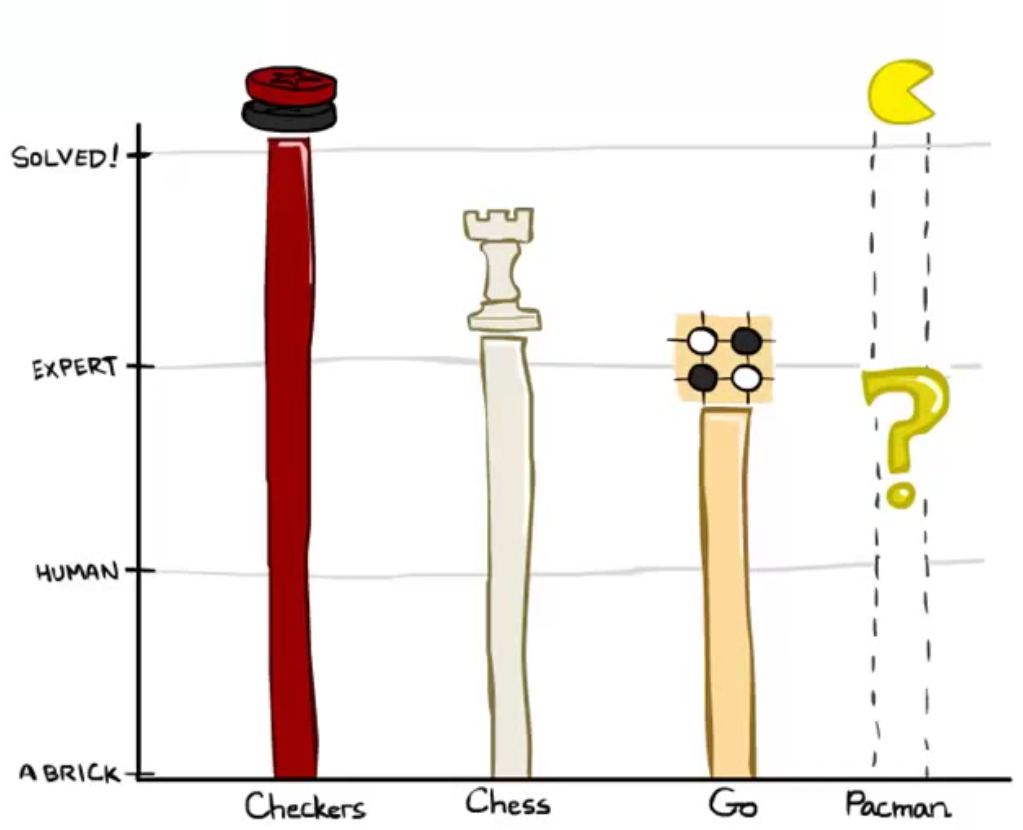
\includegraphics[height=5cm, width=6cm]{img/common-games}
\end{center}
All of the world champion agents above use, at least to some degree, the adversarial search techniques that we're about to cover. As opposed to normal search, which returned a comprehensive plan, adversarial search returns a \textbf{strategy}, or \textbf{policy}, which simply recommends the best possible move given some configuration of our agent(s) and their adversaries. We'll soon see that such algorithms have the beautiful property of giving rise to behavior through computation - the computation we run is relatively simple in concept and widely generalizable, yet innately generates cooperation between agents on the same team as well as "outthinking" of adversarial agents.

\section*{Minimax}
The first zero-sum-game algorithm we will consider is \textbf{minimax}, which runs under the motivating assumption that the opponent we face behaves optimally, and will always perform the move that is worst for us. To introduce this algorithm, we must first formalize the notion of \textbf{terminal utilities} and \textbf{state value}. The value of a state is the optimal score attainable by the agent which controls that state. In order to get a sense of what this means, observe the following trivially simple Pacman game board:
\begin{center}
	
\includegraphics{img/easy-pacman}
\end{center}
Assume that Pacman starts with 10 points and loses 1 point per move until he eats the pellet, at which point the game arrives at a \textbf{terminal state} and ends. We can start building a \textbf{game tree} for this board as follows, where children of a state are successor states just as in search trees for normal search problems:
\begin{center}
	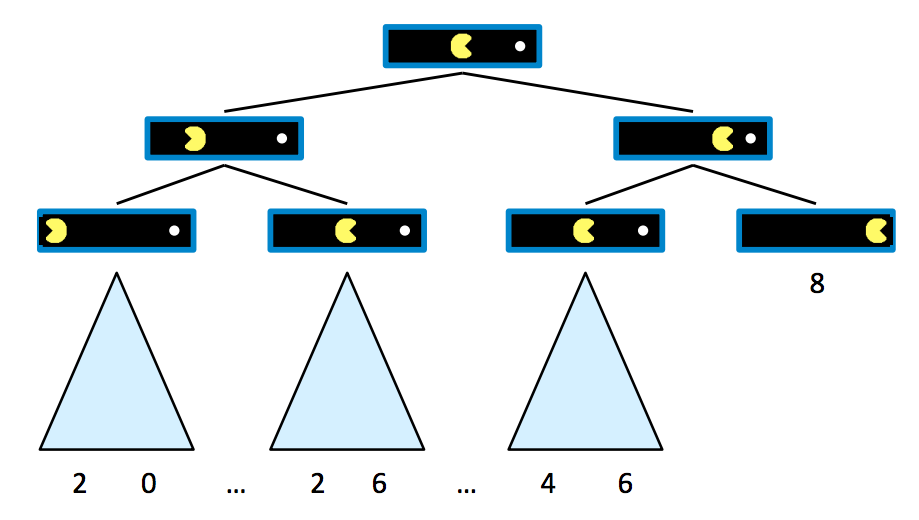
\includegraphics[width=11.2cm]{img/easy-pacman-tree}
\end{center}
It's evident from this tree that if Pacman goes straight to the pellet, he ends the game with a score of 8 points, whereas if he backtracks at any point, he ends up with some lower valued score. Now that we've generated a game tree with several terminal and intermediary states, we're ready to formalize the meaning of the value of any of these states.

A state's value is defined as the best possible outcome (\textbf{utility}) an agent can achieve from that state. We'll formalize the concept of utility more concretely later, but for now it's enough to simply think of an agent's utility as its score or number of points it attains. The value of a terminal state, called a \textbf{terminal utility}, is always some deterministic known value and an inherent game property. In our Pacman example, the value of the rightmost terminal state is simply 8, the score Pacman gets by going straight to the pellet. The value of a non-terminal state is defined as the maximum of the values of its children. Defining $V(s)$ as the function defining the value of a state $s$, we can summarize the above discussion:
	\begin{eqnarray*}
		\forall \: \text{non-terminal states},& V(s) &= \max_{s'\in successors(s)}V(s') \\
		\forall \: \text{terminal states},& V(s) &= \quad\text{known}
	\end{eqnarray*}
This sets up a very simple recursive rule, from which it should make sense that the value of the root node's direct right child will be 8, and the root node's direct left child will be 6, since these are the maximum possible scores the agent can obtain if it moves right or left, respectively, from the start state. It follows that by running such computation, an agent can determine that it's optimal to move right, since the right child has a greater value than the left child of the start state.

Let's now introduce a new game board with an adversarial ghost that wants to keep Pacman from eating the pellet. 
\begin{center}
	
\includegraphics{img/pacman-with-ghost}
\end{center}
The rules of the game dictate that the two agents take turns making moves, leading to a game tree where the two agents switch off on layers of the tree that they "control". An agent having control over a node simply means that node corresponds to a state where it is that agent's turn, and so it's their opportunity to decide upon an action and change the game state accordingly. Here's the game tree that arises from the new two-agent game board above:
\begin{center}
	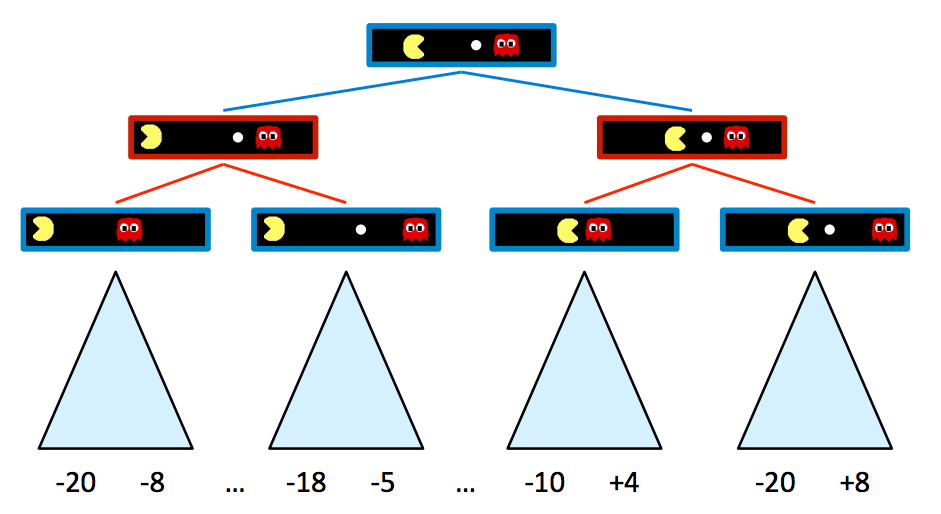
\includegraphics[width=12cm]{img/pacman-with-ghost-full-game-tree}
\end{center}
Blue nodes correspond to nodes that Pacman controls and can decide what action to take, while red nodes correspond to ghost-controlled nodes. Note that all children of ghost-controlled nodes are nodes where the ghost has moved either left or right from its state in the parent, and vice versa for Pacman-controlled nodes. For simplicity purposes, let's truncate this game tree to a depth-2 tree, and assign spoofed values to terminal states as follows:
\begin{center}
	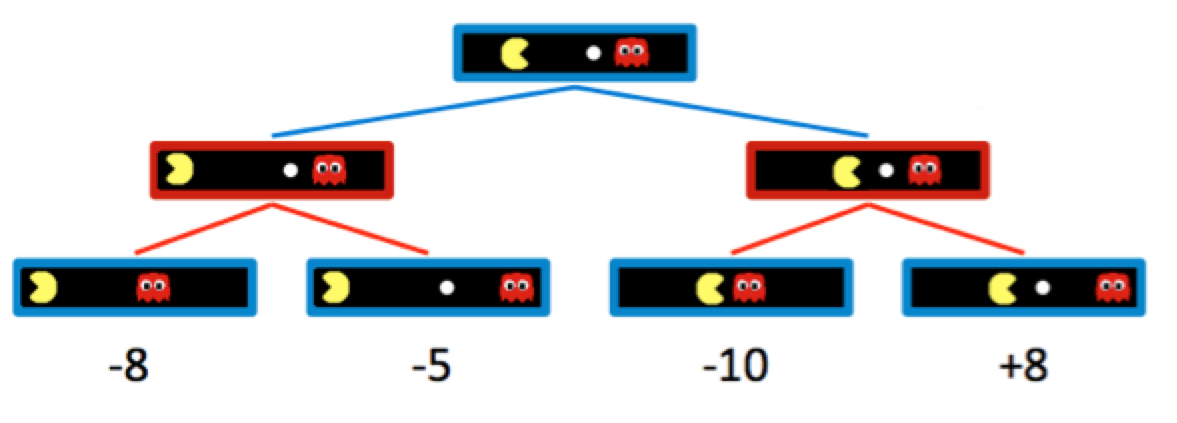
\includegraphics[width=12cm]{img/small-game-tree}
\end{center}
Naturally, adding ghost-controlled nodes changes the move Pacman believes to be optimal, and the new optimal move is determined with the minimax algorithm. Instead of maximizing over children at every level of the tree, the minimax algorithm only maximizes over the children of nodes controlled by Pacman, while minimizing over the children of nodes controlled by ghosts. Hence, the two ghost nodes above have values of $\min(-8, -5) = -8$ and $\min(-10, +8) = -10$ respectively. Correspondingly, the root node controlled by Pacman has a value of $\max(-8, -10) = -8$. Since Pacman wants to maximize his score, he'll go left and take the score of $-8$ rather than trying to go for the pellet and scoring $-10$. This is a prime example of the rise of behavior through computation - though Pacman wants the score of $+8$ he can get if he ends up in the rightmost child state, through minimax he "knows" that an optimally-performing ghost will not allow him to have it. In order to act optimally, Pacman is forced to hedge his bets and counterintuitively move away from the pellet to minimize the magnitude of his defeat. We can summarize the way minimax assigns values to states as follows:
 	\begin{eqnarray*}
		\forall \: \text{agent-controlled states},& V(s) &= \max_{s'\in successors(s)}V(s') \\
		\forall \: \text{opponent-controlled states},& V(s) &= \min_{s'\in successors(s)}V(s') \\
		\forall \: \text{terminal states},& V(s) &= \quad\text{known}
	\end{eqnarray*}
In implementation, minimax behaves similarly to depth-first search, computing values of nodes in the same order as DFS would, starting with the the leftmost terminal node and iteratively working its way rightwards. More precisely, it performs a \textbf{preorder traversal} of the game tree. The resulting pseudocode for minimax is both elegant and intuitively simple, and is presented below:
\begin{center}
	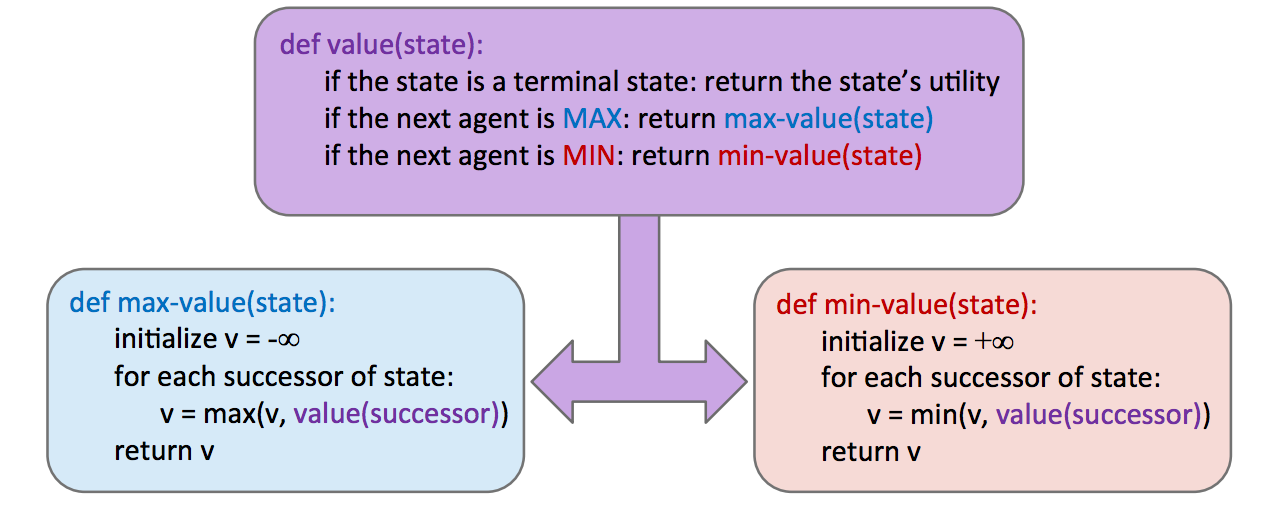
\includegraphics[width=12cm]{img/minimax-pseudocode}
\end{center} 

\subsection*{Alpha-Beta Pruning}
Minimax seems just about perfect - it's simple, it's optimal, and it's intuitive. Yet, its execution is very similar to depth-first search and it's time complexity is identical, a dismal $O(b^m)$. Recalling that $b$ is the branching factor and $m$ is the approximate tree depth at which terminal nodes can be found, this yields far too great a runtime for many games. For example, chess has a branching factor $b \approx 35$ and tree depth $m \approx 100$. To help mitigate this issue, minimax has an optimization - \textbf{alpha-beta pruning}.

Conceptually, alpha-beta pruning is this: if you're trying to determine the value of a node $n$ by looking at it's successors, stop looking as soon as you know that $n$'s value can at best equal the optimal value of $n$'s parent. Let's unravel what this tricky statement means with an example. Consider the following game tree, with square nodes corresponding to terminal states, downward-pointing triangles corresponding to minimizing nodes, and upward-pointing triangles corresponding to maximizer nodes:
\begin{center}
	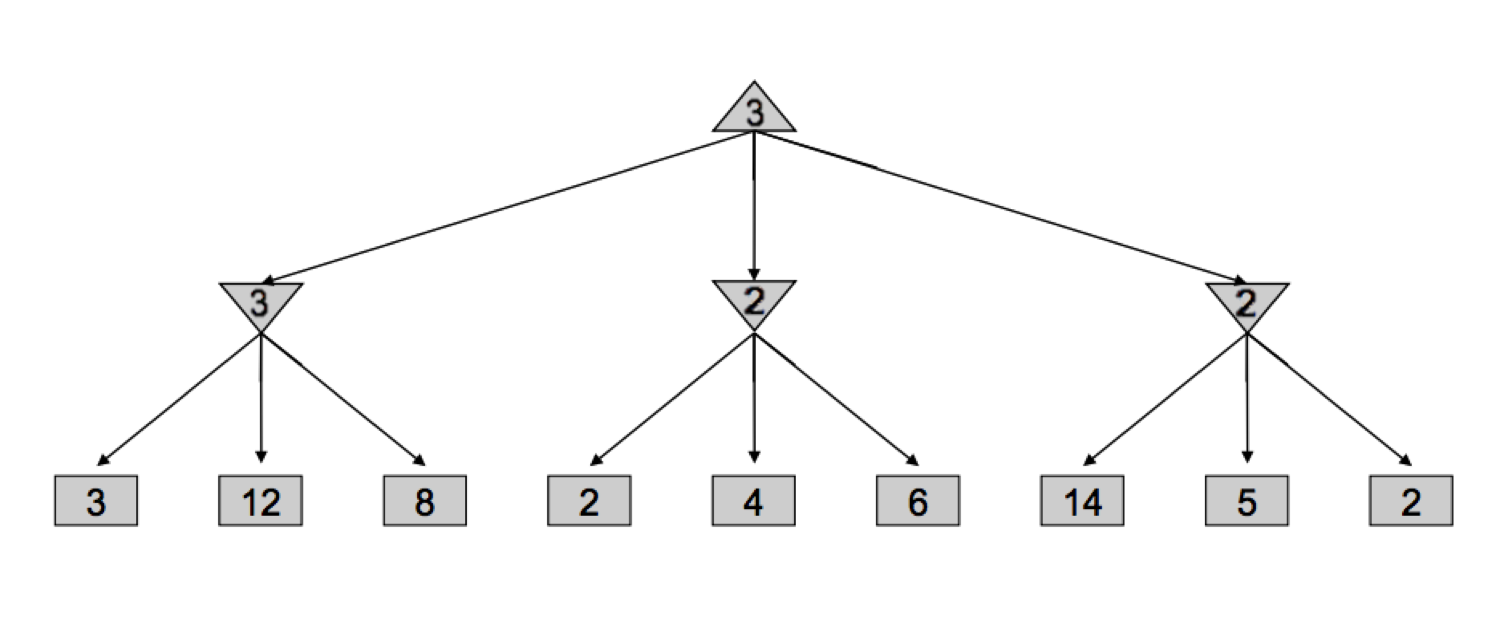
\includegraphics[width=12cm]{img/alphabeta-example-pt1}
\end{center}
Let's walk through how minimax derived this tree - it began by iterating through the nodes with values 3, 12, and 8, and assigning the value $\min(3, 12, 8) = 3$ to the leftmost minimizer. Then, it assigned $\min(2, 4, 6) = 2$ to the middle minimizer, and $\min(14, 5, 2) = 2$ to the rightmost minimizer, before finally assigning $\max(3, 2, 2) = 3$ to the maximizer at the root. However, if we think about this situation, we can come to the realization that as soon as we visit the child of the middle minimizer with value $2$, we no longer need to look at the middle minimizer's other children. Why? Since we've seen a child of the middle minimizer with value 2, we know that no matter what values the other children hold, the value of the middle minimizer can be at most 2. Now that this has been established, let's think one step further still - the maximizer at the root is deciding between the value of 3 of the left minimizer, and the value that's $\leq 2$, it's guaranteed to \textit{select the 3 returned by the left minimizer over the value returned by the middle minimizer}, regardless of the values of its remaining children. This is precisely why we can \textbf{prune} the search tree, never looking at the remaining children of the middle minimizer:
\begin{center}
	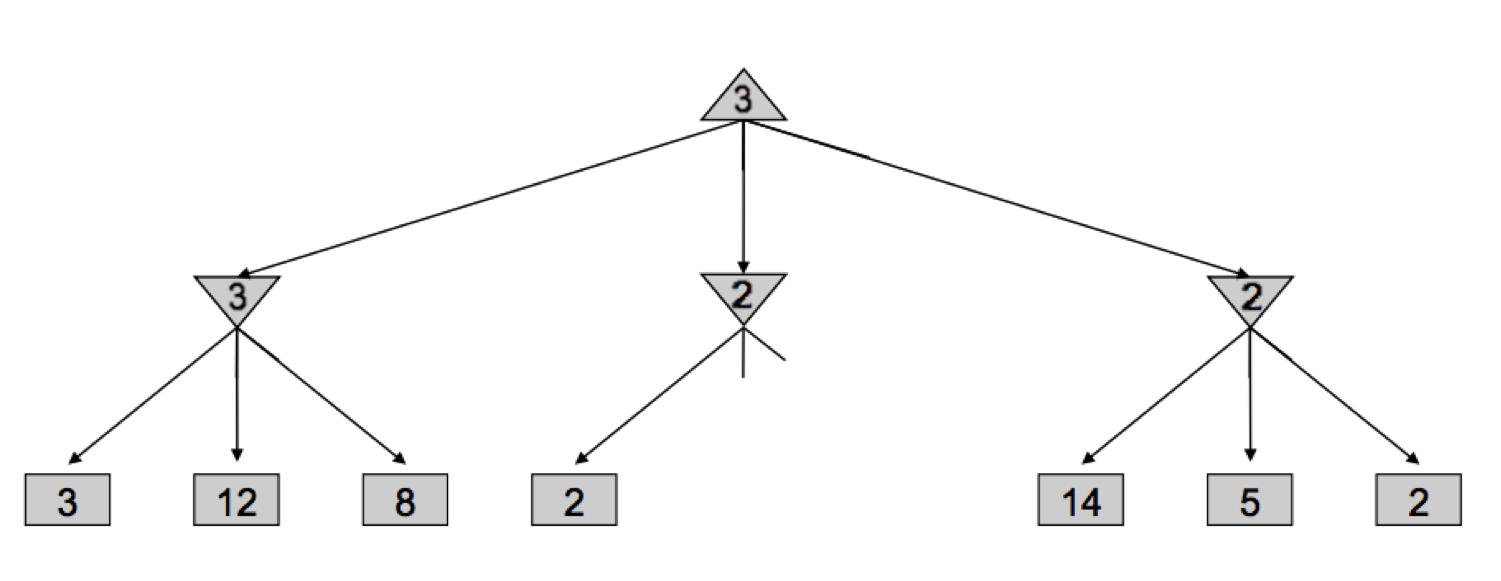
\includegraphics[width=12cm]{img/alphabeta-example-pt2}
\end{center}
Implementing such pruning can reduce our runtime to as good as $O(b^{m/2})$, effectively doubling our "solvable" depth. In practice, it's often a lot less, but generally can make it feasible to search down to at least one or two more levels. This is still quite significant, as the player who thinks 3 moves ahead is favored to win over the player who thinks 2 moves ahead. This pruning is exactly what the minimax algorithm with alpha-beta pruning does, and is implemented as follows:
\begin{center}
	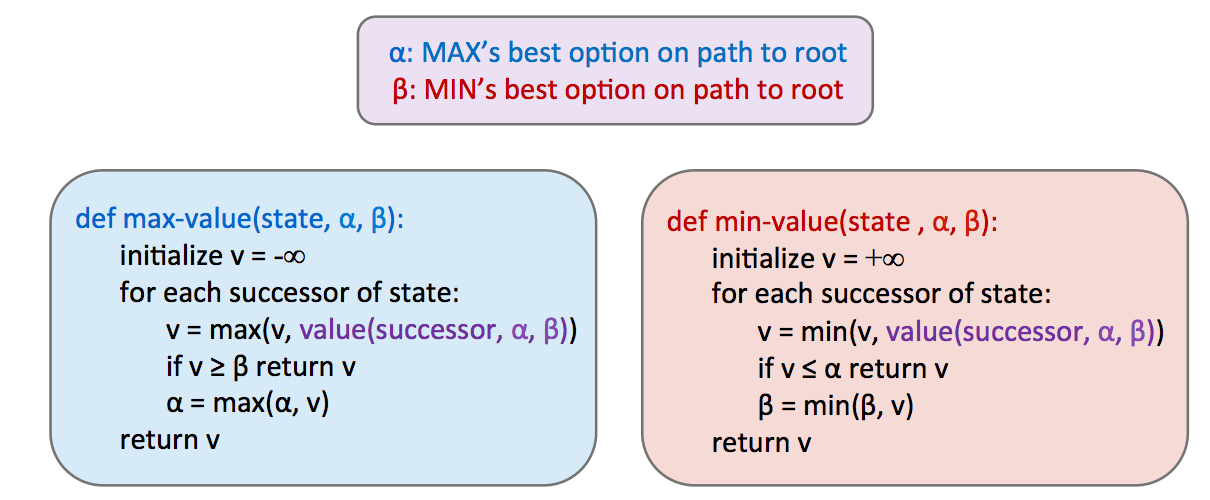
\includegraphics[width=12cm]{img/alphabeta-pseudo}
\end{center}
Take some time to compare this with the pseudocode for vanilla minimax, and note the differences.

<PROPERTIES OF ALPHABETA>

\subsection*{Evaluation Functions}
Though alpha-beta pruning can help increase the depth for which we can feasibly run minimax, this still usually isn't even close to good enough to get to the bottom of search trees for a large majority of games. As a result, we turn to \textbf{evaluation functions}, functions that take in a state and output an estimate of the true minimax value of that node. Typically, this is plainly interpreted as "better" states being assigned higher values by a good evaluation function than "worse" states. Evaluation functions are widely employed in \textbf{depth-limited minimax}, where we treat non-terminal nodes located at our maximum solvable depth as terminal nodes, giving them mock terminal utilities as determined by a carefully selected evaluation function. Because evaluation functions can only yield estimates of the values of non-terminal utilities, this removes the guarantee of optimal play when running minimax. 

A lot of thought and experimentation is typically put into the selection of an evaluation function when designing an agent that runs minimax, and the better the evaluation function is, the closer the agent will come to behaving optimally. Additionally, going deeper into the tree before using an evaluation function also tends to give us better results - burying their computation deeper in the game tree mitigates the compromising of optimality. These functions serve a very similar purpose in games as heuristics do in standard search problems.

The most common design for an evaluation function is a weighted linear combination of \textbf{features}.
$$Eval(s) = w_1f_1(s) + w_2f_2(s) + ... + w_nf_n(s)$$
 Each $f_i(s)$ corresponds to a feature extracted from the input state $s$, and each feature is assigned a corresponding \textbf{weight} $w_i$. Features are simply some element of a game state that we can extract and assign a numerical value. For example, in a game of checkers we might construct an evaluation function with 4 features: number of agent pawns, number of agent kings, number of opponent pawns, and number of opponent kings. We'd then select appropriate weights based loosely on their importance. In our checkers example, it makes most sense to select positive weights for our agent's pawns/kings and negative weights for our opponents pawns/kings. Furthermore, we might decide that since kings are more valuable pieces in checkers than pawns, the features corresponding to our agent's/opponent's kings deserve weights with greater magnitude than the features concerning pawns. Below is a possible evaluation function that conforms to the features and weights we've just brainstormed:
 $$Eval(s) = 2 \cdot agent\_kings(s) + agent\_pawns(s) - 2 \cdot opponent\_kings(s) - opponent\_pawns(s)$$
 As you can tell, evaluation function design can be quite free-form. The most important thing to keep in mind is that the evaluation function yields higher scores for better positions as frequently as possible. This may require a lot of fine-tuning and experimenting on the performance of agents using evaluation functions with a multitude of different features and weights.

\section*{Expectimax}
We've now seen how minimax works and how running full minimax allows us to respond optimally against an optimal opponent. However, minimax has some natural constraints on the situations to which it can respond. Because minimax believes it is responding to an optimal opponent, it's often overly pessimistic in situations where optimal responses to an agent's actions are not guaranteed. Such situations include scenarios with inherent randomness such as card or dice games or unpredictable opponents that move randomly or suboptimally. We'll talk about scenarios with inherent randomness much more in detail when we discuss \textbf{Markov decision processes} in the next note. 

This randomness can be represented through a generalization of minimax known as \textbf{expectimax}. Expectimax introduces \textit{chance nodes} into the game tree, which instead of considering the worst case scenario as minimizer nodes do, considers the \textit{average case}. More specifically, while minimizers simply compute the minimum utility over their children, chance nodes compute the \textbf{expected utility} or expected value. Our rule for determining values of nodes with expectimax is as follows:
	\begin{eqnarray*}
		\forall \: \text{agent-controlled states},& V(s) &= \max_{s'\in successors(s)}V(s') \\
		\forall \: \text{chance states},& V(s) &= \sum_{s'\in successors(s)}p(s')V(s') \\
		\forall \: \text{terminal states},& V(s) &= \quad\text{known}
	\end{eqnarray*}
In the above formulation, $p(s')$ refers to either the probability that a given probabilistic action results in state $s'$, or the probability that an opponent chooses an action that results in $s'$, depending on the specifics of the game and the game tree under consideration. From this definition, we can see that minimax is simply a special case of expectimax. Minimizer nodes are simply chance nodes that assign a probability of 1 to their lowest-value child and probability 0 to all other children. In general, probabilities are selected to properly reflect the game state we're trying to model, but we'll cover how this process works in more detail in future notes. For now, it's fair to assume that these probabilities are simply inherent game properties.

The pseudocode for expectimax is quite similar to minimax, with only a few small tweaks to account for expected utility instead of minimum utility, since we're replacing minimizing nodes with chance nodes:
\begin{center}
	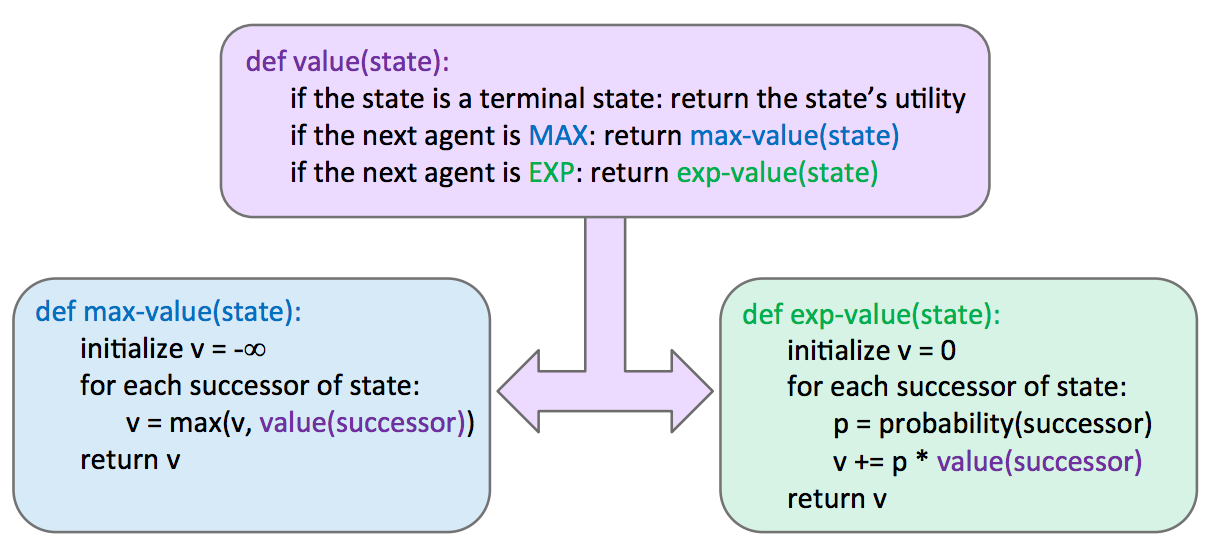
\includegraphics[width=12cm]{img/expectimax-pseudocode}
\end{center}
Before we continue, let's quickly step through a simple example. Consider the following expectimax tree, where chance nodes are represented by circular nodes instead of the upward/downward facing triangles for maximizers/minimizers.
\begin{center}
	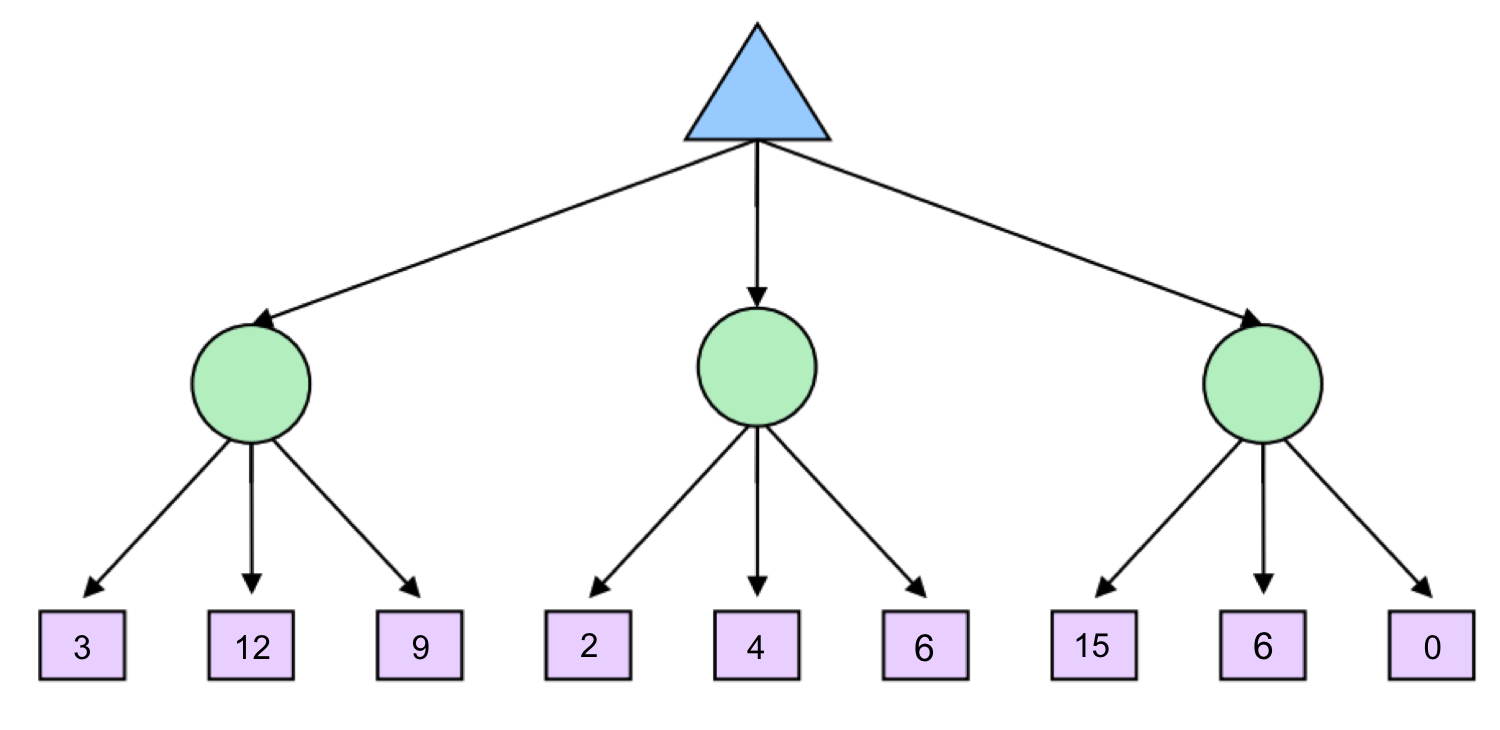
\includegraphics[width=12cm]{img/unfilled-expectimax}
\end{center}
Assume for simplicity that all children of each chance node have a probability of occurrence of $\frac{1}{3}$. Hence, from our expectimax rule for value determination, we see that from left to right the 3 chance nodes take on values of $\frac{1}{3} \cdot 3 + \frac{1}{3} \cdot 12 + \frac{1}{3} \cdot 9 = \boxed{8}$, $\frac{1}{3} \cdot 2 + \frac{1}{3} \cdot 4 + \frac{1}{3} \cdot 6 = \boxed{4}$, and $\frac{1}{3} \cdot 15 + \frac{1}{3} \cdot 6 + \frac{1}{3} \cdot 0 = \boxed{7}$. The maximizer selects the maximimum of these three values, $\boxed{8}$, yielding a filled-out game tree as follows:
\begin{center}
	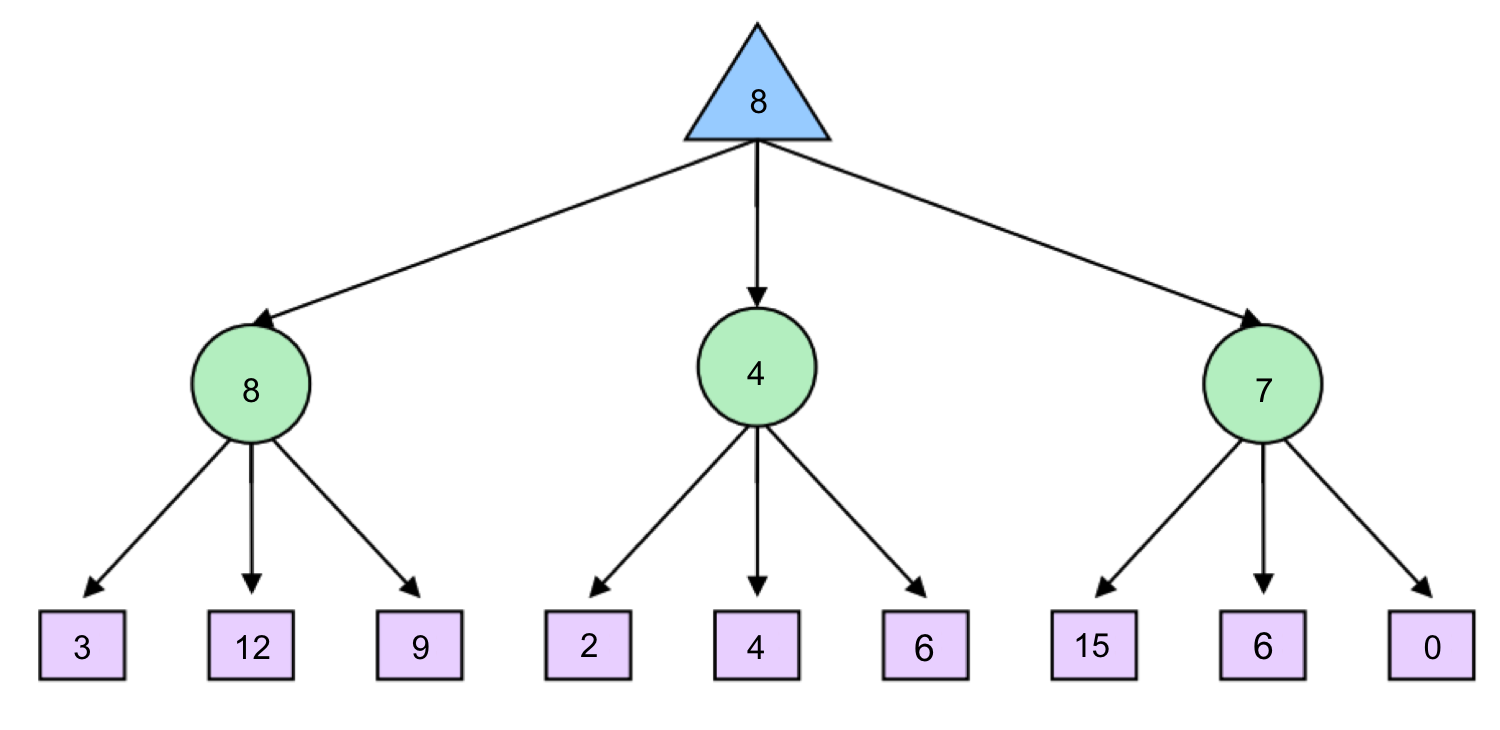
\includegraphics[width=12cm]{img/filled-expectimax}
\end{center}
As a final note on expectimax, it's important to realize that it's always necessary to look at all children of chance nodes - we can never terminate early and prune like in minimax. Unlike when computing minimums or maximums in minimax, a single value can skew the expected value computed by expectimax arbitrarily high or low.

\subsection*{Mixed Layer Types}
Though minimax and expectimax call for alternating maximizer/minimizer nodes and maximizer/chance nodes respectively, many games still don't follow the exact pattern of alternation that these two algorithms mandate. Even in Pacman, after Pacman moves, there are usually multiple ghosts that take turns making moves, not a single ghost. We can account for this by very fluidly adding layers into our game trees as necessary. In the Pacman example for a game with four ghosts, this can be done by having a maximizer layer followed by 4 consecutive ghost/minimizer layers before the second Pacman/maximizer layer. In fact, doing so inherently gives rise to cooperation across all minimizers, as they alternatively take turns further minimizing the utility attainable by the maximizer(s). It's even possible to combine chance node layers with both minimizers and maximizers. If we have a game of Pacman with two ghosts, where one ghost behaves randomly and the other behaves optimally, we could simulate this with alternating groups of maximizer-chance-minimizer nodes.
\begin{center}
	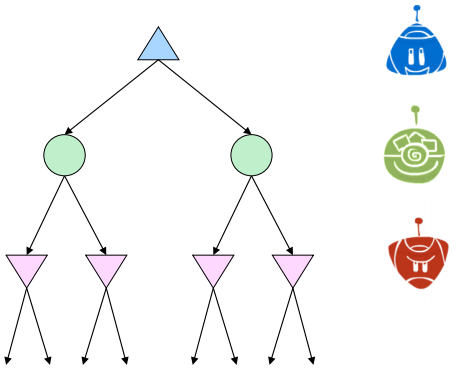
\includegraphics[width=6cm]{img/mixed-layer}
\end{center}
As is evident, there's quite a bit of room for robust variation in node layering, allowing development of game trees and adversarial search algorithms that are modified expectimax/minimax hybrids for any zero-sum game.

\section*{General Games}
Not all games are zero-sum. Indeed, different agents may have have distinct tasks in a game that don't directly involve strictly competing with one another. Such games can be set up with trees characterized by \textbf{multi-agent utilities}. Such utilities, rather than being a single value that alternating agents try to minimize or maximize, are represented as tuples with different values within the tuple corresponding to unique utilities for different agents. Each agent then attempts to maximize their own utility at each node they control, ignoring the utilities of other agents. Consider the following tree:
\begin{center}
	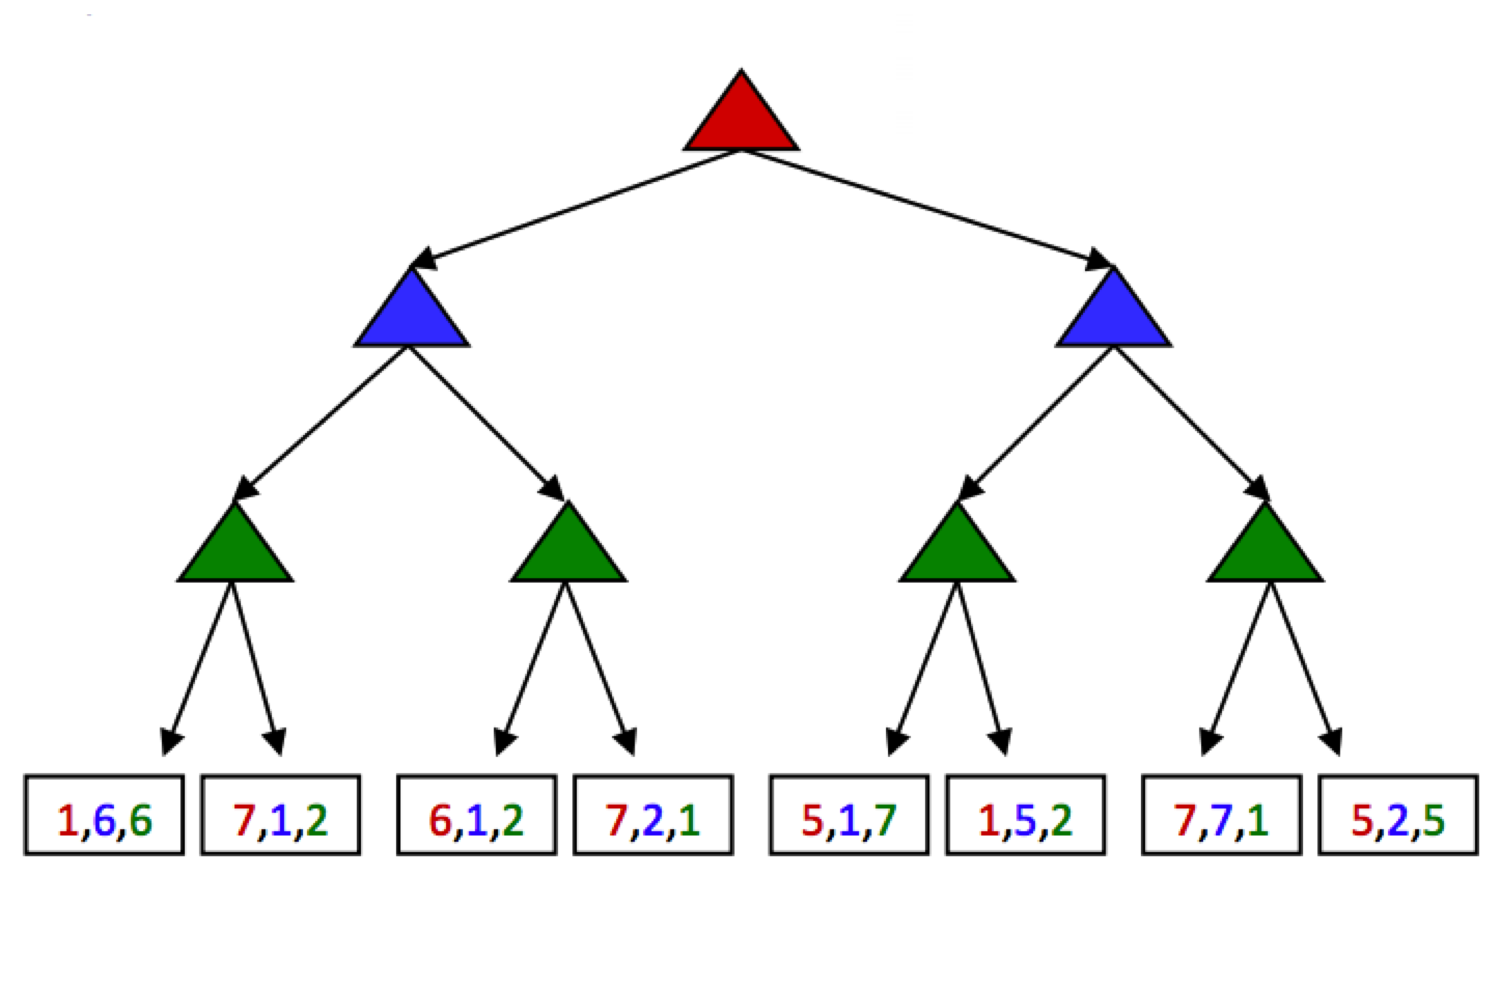
\includegraphics[width=12cm]{img/multi-agent-utility}
\end{center}
The red, green, and blue nodes correspond to three separate agents, who maximize the red, green, and blue utilities respectively out of the possible options in their respective layers. Working through this example ultimately yields the utility tuple $(5, 2, 5)$ at the top of the tree. General games with multi-agent utilities are a prime example of the rise of behavior through computation, as such setups invoke cooperation since the utility selected at the root of the tree tends to yield a reasonable utility for all participating agents.

\section*{Utilities}
Thoughout our discussion of games, the concept of utility has come up repeatedly. Utility values are generally hard-wired into games, and agents run some variation of the algorithms discussed in this note to select an action. We'll now discuss what's necessary in order to generate a viable utility function. 

Rational agents must follow the \textbf{principle of maximum utility} - they must always select the action that maximizes their expected utility. However, obeying this principle only benefits agents that have \textbf{rational preferences}. To construct an example of irrational preferences, say there exist 3 objects, $A$, $B$, and $C$, and our agent is currently in possession of $A$. Say our agent has the following set of irrational preferences:
	\begin{itemize}
		\item Our agent prefers $B$ to $A$ plus \$1
		\item Our agent prefers $C$ to $B$ plus \$1
		\item Our agent prefers $A$ to $C$ plus \$1
	\end{itemize}
A malicious agent in possession of $B$ and $C$ can trade our agent $B$ for $A$ plus a dollar, then $C$ for $B$ plus a dollar, then $A$ again for $C$ plus a dollar. Our agent has just lost \$3 for nothing! In this way, our agent can be forced to give up all of its money in an endless and nightmarish cycle.

Let's now properly define the mathematical language of preferences:
	\begin{itemize} 
		\item If an agent prefers receiving a prize $A$ to receiving a prize $B$, this is written $A \succ B$
		\item If an agent is indifferent between receiving $A$ or $B$, this is written as $A \sim B$
		\item A \textbf{lottery} is a situation with different prizes resulting with different probabilities. To denote lottery where $A$ is received with probability $p$ and $B$ is received with probability $(1-p)$, we write $$L = [p,\: A;\:\:(1-p),\: B]$$
	\end{itemize}
In order for a set of preferences to be rational, they must follow the five \textbf{Axioms of Rationality}:
	\begin{itemize}
		\item \textit{Orderability}: \tab$(A \succ B) \vee (B \succ A) \vee (A \sim B)$ \\
			\tab\tab A rational agent must either prefer one of $A$ or $B$, or be indifferent between the two.
		\item \textit{Transitivity}: \tab$(A \succ B) \wedge (B \succ C) \Rightarrow (A \succ C)$ \\
			\tab\tab If a rational agent prefers $A$ to $B$ and $B$ to $C$, then it prefers $A$ to $C$.
		\item \textit{Continuity}: \tab$A \succ B \succ C \Rightarrow \exists{p} \: [p,\: A; \:\: (1-p),\: C] \sim B$ \\
			\tab\tab If a rational agent prefers $A$ to $B$ but $B$ to $C$, then it's possible to construct a lottery $L$ between $A$ \\
			\tab\tab and $C$ such that the agent is indifferent between $L$ and $B$ with appropriate selection of $p$.
		\item \textit{Substitutability}: \tab$A \sim B \Rightarrow [p,\: A; \:\: (1-p),\: C] \sim [p,\: B; \:\: (1-p),\: C]$ \\
			\tab\tab A rational agent indifferent between two prizes $A$ and $B$ is also indifferent between any two \\
			\tab\tab lotteries which only differ in substitutions of $A$ for $B$ or $B$ for $A$.
		\item \textit{Monotonicity}: \tab$A \succ B \Rightarrow (p \geq q \Leftrightarrow [p,\: A; \:\: (1-p),\: B] \succeq [q,\: A; \:\: (1-q),\: B]$ \\
			\tab\tab If a rational agent prefers $A$ over $B$, then given a choice between lotteries involving only $A$ and $B$, \\ 
			\tab\tab the agent prefers the lottery assigning the highest probability to $A$. 
	\end{itemize}
If all five axioms are satisfied by an agent, then it's guaranteed that the agent's behavior is describable by maximizing its expected utility. More specifically, this implies that there exists a real-valued utility function $U$ that when implemented will assign greater utilities to preferred prizes, and also that the utility of a lottery is the expected value of the utility of the prize resulting from the lottery. These two statements can be summarized in two concise mathematical equivalences:
	\begin{eqnarray}
		U(A) \geq U(B) &\Leftrightarrow& A \succeq B \\
		U([p_1,\: S_1;\:\: ... \:\: ;p_n,\:S_n]) &=& \sum_ip_iU(S_i)
	\end{eqnarray} 
If these constraints are met and an appropriate choice of algorithm is made, the agent implementing such a utility function is guaranteed to behave optimally. 





\end{document}